\documentclass[a4paper,10pt]{article}

%%%%%%%%%%%%%%%%%%%%%%%%%%%%%%%%%%%%%%%%%%%%%%%%%%
% Los paquetes permiten ampliar las capacidades de LaTeX.                     %
%%%%%%%%%%%%%%%%%%%%%%%%%%%%%%%%%%%%%%%%%%%%%%%%%%
% Paquete para inclusión de gráficos.
\usepackage{graphicx}

% Paquete para definir la codificación del conjunto de caracteres usado
\usepackage[utf8]{inputenc}

% Paquete para definir el idioma usado.
\usepackage[spanish]{babel}

% Paquete para introducir codigo de programacion
\usepackage{listings}

 % Para poder introducir otrod PDFs
\usepackage{pdfpages}

% Para inseratar imagenes
\usepackage{graphicx}
\usepackage{subfigure}

%\usepackage{mips}



% Título principal del documento.
\title{\textbf{Trabajo práctico 3: Datapath}}


% Información sobre los autores.
\author{Augusto Arturi (\#97498)\\
\texttt{turitoh@gmail.com}\\
\\
Matias Rozanec (\#97404)\\            \texttt{rozanecm@gmail.com}\\
\\
Agustin Miguel Payaslian (\#96885)\\            \texttt{payas17@hotmail.com}\\
\\
\normalsize{Grupo Nro. \# - 2do. Cuatrimestre de 2017}\\
\\
\\
\normalsize{66.20 Organización de Computadoras}\\
\normalsize{Facultad de Ingeniería, Universidad de Buenos Aires}\\
}
\date{30.nov.2017}

\lstset{
  language=bash,
  basicstyle=\ttfamily
}
\lstdefinestyle{numbers} {numbers=left, stepnumber=1, numberstyle=\tiny, numbersep=10pt}

\lstdefinestyle{MyFrame}{backgroundcolor=\color{white},frame=shadowbox}

\lstdefinestyle{noframe} {language=bash,style=MyFrame,frame=none}

\lstdefinestyle{customc}{
  belowcaptionskip=1\baselineskip,
  breaklines=true,  
  xleftmargin=-5em,
  language=C,
  showstringspaces=false,
  basicstyle=\footnotesize\ttfamily,
  keywordstyle=\bfseries\color{green!40!black},
  commentstyle=\itshape\color{purple!40!black},
  identifierstyle=\color{blue},
  stringstyle=\color{orange},
  numberstyle=\tiny,
  resetmargins=true,
  style=MyFrame,
  numbers=left,                   % where to put the line-numbers
  numberstyle=\tiny\color{gray},
}

\lstdefinestyle{customasm}{
  belowcaptionskip=1\baselineskip,
  frame=L,
  xleftmargin=-5em,
  language=[x86masm]Assembler,
  basicstyle=\footnotesize\ttfamily,
  commentstyle=\itshape\color{purple!40!black},
  style=MyFrame,
}

\definecolor{dkgreen}{rgb}{0,0.6,0}
\definecolor{gray}{rgb}{0.5,0.5,0.5}
\definecolor{mauve}{rgb}{0.58,0,0.82}

\lstdefinestyle{mips}{ %
  language=[mips]Assembler,       % the language of the code
  basicstyle=\footnotesize,       % the size of the fonts that are used for the code
  numbers=left,                   % where to put the line-numbers
  numberstyle=\tiny\color{gray},  % the style that is used for the line-numbers
  stepnumber=1,                   % the step between two line-numbers. If it's 1, each line 
                                  % will be numbered
  numbersep=5pt,                  % how far the line-numbers are from the code
  backgroundcolor=\color{white},  % choose the background color. You must add \usepackage{color}
  showspaces=false,               % show spaces adding particular underscores
  showstringspaces=false,         % underline spaces within strings
  showtabs=false,                 % show tabs within strings adding particular underscores
  frame=single,                   % adds a frame around the code
  rulecolor=\color{black},        % if not set, the frame-color may be changed on line-breaks within not-black text (e.g. commens (green here))
  tabsize=4,                      % sets default tabsize to 2 spaces
  captionpos=b,                   % sets the caption-position to bottom
  breaklines=true,                % sets automatic line breaking
  breakatwhitespace=false,        % sets if automatic breaks should only happen at whitespace
  title=\lstname,                 % show the filename of files included with \lstinputlisting;
    xleftmargin=-5em,                                % also try caption instead of title
  keywordstyle=\color{blue},          % keyword style
  commentstyle=\color{dkgreen},       % comment style
  stringstyle=\color{mauve},         % string literal style
  escapeinside={\%*}{*)},            % if you want to add a comment within your code
  morekeywords={*,...}   
            % if you want to add more keywords to the set
}


\begin{document}


% Inserta el título.
\maketitle
% Quita el número en la primer página.

% Resumen

\begin{figure}[!htp]
\centering

\includegraphics[scale=1]{fiuba_logo.png} 

\end{figure}
\thispagestyle{empty}
\newpage

\begin{abstract}
El objetivo del presente trabajo es familiarizarse con la arquitectura de una CPU MIPS, específicamente con el datapath y la implementación de instrucciones. Para ello se agregarán diversas instrucciones de CPU provistas por el simulador DrMIPS.
\end{abstract}


\section{Introducción}
Aquí se comenta en forma escueta cómo está constituido el presente informe, donde  básicamente  se  encuentran  dos  secciones  principales: Desarrollo y Conclusiones.\\
En Desarrollo se encuentran breves comentarios sobre la implementacion de las distintas instrucciones. En la seccion conclusiones se discuten los resultados obtenidos.

\section{Desarrollo}

\subsection{Implementación}
Para cada una de las instrucciones a agregar, lo primero que se estudió fue el código de la instrucción. De esta forma, se pudo escribir la instrucción en el archivo .set correspondiente al datapath que se pedía modificar. Una vez agregada la instrucción en el archivo .set, se procedió a analizar la arquitectura. En base a este análisis se pudo ver qué modificaciones había que llevar adelante en el datapath para que la instrucción agregada efectivamente haga lo que debe hacer.

\subsection{Agregado de instrucciones}
En todos los casos, los códigos específicos de cada instrucción han sido consultados en manuales y bibliografía autorizada. 
\subsubsection{Instrucciones \texttt{sll} y \texttt{srl} en el datapath \texttt{pipeline.cpu}}
Para agregar estas dos instrucciones, se debieron agregar las siguientes líneas: 
\begin{lstlisting}[breaklines=true]
"sll":  {"type": "R", "args": ["reg", "reg", "int"], "fields": {"op": 0, "rs": "#2", "rt": "#3", "rd": "#1", "shamt": "#3", "func": 0}}


"srl":  {"type": "R", "args": ["reg", "reg", "int"], "fields": {"op": 0, "rs": "#2", "rt": "#3", "rd": "#1", "shamt": "#3", "func": 2}}
\end{lstlisting}
En ambos casos se trata de instrucciones de tipo \texttt{R}, cuyo \texttt{opcode} es 0, y cuyos argumentos 1, 2 y 3 corresponden a los registros \texttt{rd}, \texttt{rs} y \texttt{shamt} respectivamente. En el caso de \texttt{sll}, \texttt{func} recibe el valor 0, mientras que en el caso de \texttt{srl}, este código es 2. \\
Lugo hubo que vincular los códigos de función con las operaciones de la ALU propiamente dicho. Esto se logra mediantes las siguientes líneas:\\
En la sección de control de la ALU:
\begin{lstlisting}
{"aluop": 2, "func": 0,  "out": {"Operation": 13}}
{"aluop": 2, "func": 2,  "out": {"Operation": 14}}
\end{lstlisting}
En la sección de operaciones de la ALU:
\begin{lstlisting}
"13": "sll"
"14": "srl"
\end{lstlisting}

\subsubsection{Instrucción \texttt{blt} en el datapath \texttt{pipeline.cpu}}
Esta vez se agregó la instrucción como pseudo instrucción. Esto es porque la arquitectura no puede ser modificada de forma que se pueda soportar esta operación. Las pseudo instrucciones son muy útiles a pesar de no ser implementeadas nativamente, ya que le simplifican mucho las tareas al programador. Cada pseudo instrucción está compuesta por varias instrucciones que sí están implementadas en hardware nativament. \\
Para agregar esta pseudo instrucción, se debió agregar la siguiente línea. 
\begin{lstlisting}[breaklines=true]
"blt":  {"args": ["reg", "reg", "offset"], "to": ["slt $1, #1, #2", "bne $1, $0, #3"]}
\end{lstlisting}

\subsubsection{Instrucción \texttt{j} en el datapath \texttt{unicycle.cpu}}
\begin{lstlisting}[breaklines=true]
"j":    {"type": "J", "args": ["target"], "fields": {"op": 2, "target": "#1"}, "desc": "PC = target"}
\end{lstlisting}
Esta instrucción ya se encontraba implementada en el datapath sugerido. \\
En cuanto al análisis de hazards, se llegó a la conclusión de que no es posible que en este datapath haya hazards, debido a que todo ocurre en un solo ciclo. Los hazards ocurren en sistemas con pipeline, donde una instrucción depende del resultado de otra previa de una forma en que ésta esté expuesta por el solapamiento de instrucciones en el pipeline. Como en este caso no hay pipeline, no pueden ocurrir hazards.

\subsubsection{Instrucción \texttt{jr} en el datapath \texttt{pipeline.cpu}}
En este caso se trata de una operación de tipo \texttt{R}, cuyo \texttt{opcode} es 0, y su número de función es 8. El argumento que recibe corresponde a los bits del registro \texttt{rs}. \\
Para agregar la instrucción, hubo que agregar la siguiente línea en el archivo .set correspondiente: 
Para agregar esta pseudo instrucción, se debió agregar la siguiente línea. 
\begin{lstlisting}[breaklines=true]
"jr":   {"type": "R", "args": ["reg"], "fields": {"op": 0, "rs": "#1", "rt": "0", "rd": "0", "shamt": 0, "func": 8}, "desc": "The jr instruction loads the PC register with a value stored in a register."},
\end{lstlisting}

\subsubsection{Instrucción \texttt{jalr} en el datapath \texttt{pipeline.cpu}}
Formato de la instrucci\'on:\\
\texttt{JALR rs} (\texttt{rd} = 31 implied)\\
\texttt{JALR rd, rs}\\
Descripci\'on:\\
$rd \leftarrow return\_addr, PC \leftarrow rs$\\
En este caso se vuelve a tratar de una pseudo instrucción. Ésta es compuesta por las operaciones \texttt{addi} y \texttt{jr}, ésta última implementada anteriormente.\\
La instrucci\'on completa es: \texttt{jalr rd, rs}. En caso de omitir el campo \texttt{rd}, se tomar\'a su valor como igual a 31. Como ac\'a hay dos casos posibles, hubo que agregar dos l\'ineas en el apartado de pseudo instrucciones en el archivo .set. 
\begin{lstlisting}[breaklines=true]
"jalr": {"args": ["reg", "reg"], "to": ["addi #1, $0, $ra", "jr #2"]},


"jalr": {"args": ["reg"], "to": ["addi 31, $0, $ra", "jr #1"]}
\end{lstlisting}




\subsection{Modificaciones en el datapath}
\subsubsection{Instrucciones \texttt{sll} y \texttt{srl} en el datapath \texttt{pipeline.cpu}}
Para agregar estas instrucciones, el problema que se presentó fue que la arquitectura no estaba preparada para enviarle a la alu los bits \texttt{shamt} desde el código de instrucción correspondiente a las instrucciones de bit shifting (que son 6 en total: \texttt{sll}, \texttt{srl}, \texttt{sra}, \texttt{sllv}, \texttt{srlv} y \texttt{srav}). Por lo tanto, hubo que modificar el datapath de forma que la ALU pueda recibir dichos bits. \\
Lo primero que se hizo, es agregar los cables necesarios para hacer llegar los bits de \texttt{shamt} hasta la ALU. Como \'estos son solo 5 y la ALU  recibe 32 por entrada, hubo que agregar otros (32-5) bits y concatenarlos con los 5 que quer\'iamos hacer entrar. Esto se realiz\'o mediante un generador de un valor constante (componente \texttt{Constant} de tamaño (32-5), con todos los bits en 0) y un \texttt{Concatenator}, que concatena todos los bits, obteniendo as\'i el valor de \texttt{shamt} pero en 32 bits, listo para entrar a la ALU. \\
Como la ALU  no puede recibir una entrada m\'as, hubo que agregar un multiplexor que permita seleccionar si permitir entrar la entrada que ya est\'a conectada en este momento o la entrada con el valor de \texttt{shamt}. Para lograr esto, se cable\'o la salida del multiplexor \texttt{MuxReg} a la entrada 0 del nuevo multiplexor, \texttt{MuxShamt}. A la otra entrada de este multiplexor se cable\'o el valor de \texttt{shamt}. La salida de este nuevo multiplexor se conecta a la entrada de la ALU que qued\'o libre anteriormente. \\
Queda ahora para resolver qu\'e usar como selector de este multiplexor.\\
Los bits de \texttt{shamt} deben entrar en la ALU  \'unicamente cuando se trata de operaciones de bit shifting. Para esto hay que tener en cuenta los siguientes códigos: \texttt{opcode} y \texttt{func}. \\
\texttt{opcode} es 0 para todas las instrucciones de tipo \texttt{R} menos una. Los c\'odigos \texttt{func} tienen los 3 bits m\'as significativos en 0 en todos los casos de operaciones de bit shifting. Para implementar el selector del nuevo multiplexor se utilizaron compuertas tipo \texttt{or} y \texttt{not} sobre los bits mencionados. 

\subsubsection{Instrucción \texttt{blt} en el datapath \texttt{pipeline.cpu}}
Al agregase como una pseudo Instrucci\'on, no hubo que realizar modificaciones en el datapath. 

\subsubsection{Instrucción \texttt{j} en el datapath \texttt{unicycle.cpu}}
Como se mencionó anteriormente, esta instrucción ya estaba incluída, por lo que no hubo que realizar modificaciones. 

\subsubsection{Instrucción \texttt{jr} en el datapath \texttt{pipeline.cpu}}
En este caso hubo que considerar una entrada alternativa al Program Counter, por lo que se agregó un multiplexor que recibía por una entrada lo que hasta ahora recibía el Program Counter, y por la otra el valor del registro que contiene la direcci\'on a la que nos interesa ir. La salida de este multiplexor va a la entrada del Program Counter. Mediante el uso de compuertas \texttt{or} y \texttt{not}, estudiando el c\'odigo de operaci\'on correspondiente a esta instrucci\'on, se implement\'o el selector de este nuevo multiplexor. 

\subsubsection{Instrucción \texttt{jalr} en el datapath \texttt{pipeline.cpu}}
Al agregase como una pseudo Instrucci\'on, no hubo que realizar modificaciones en el datapath. 

\newpage

\section{Conclusiones}

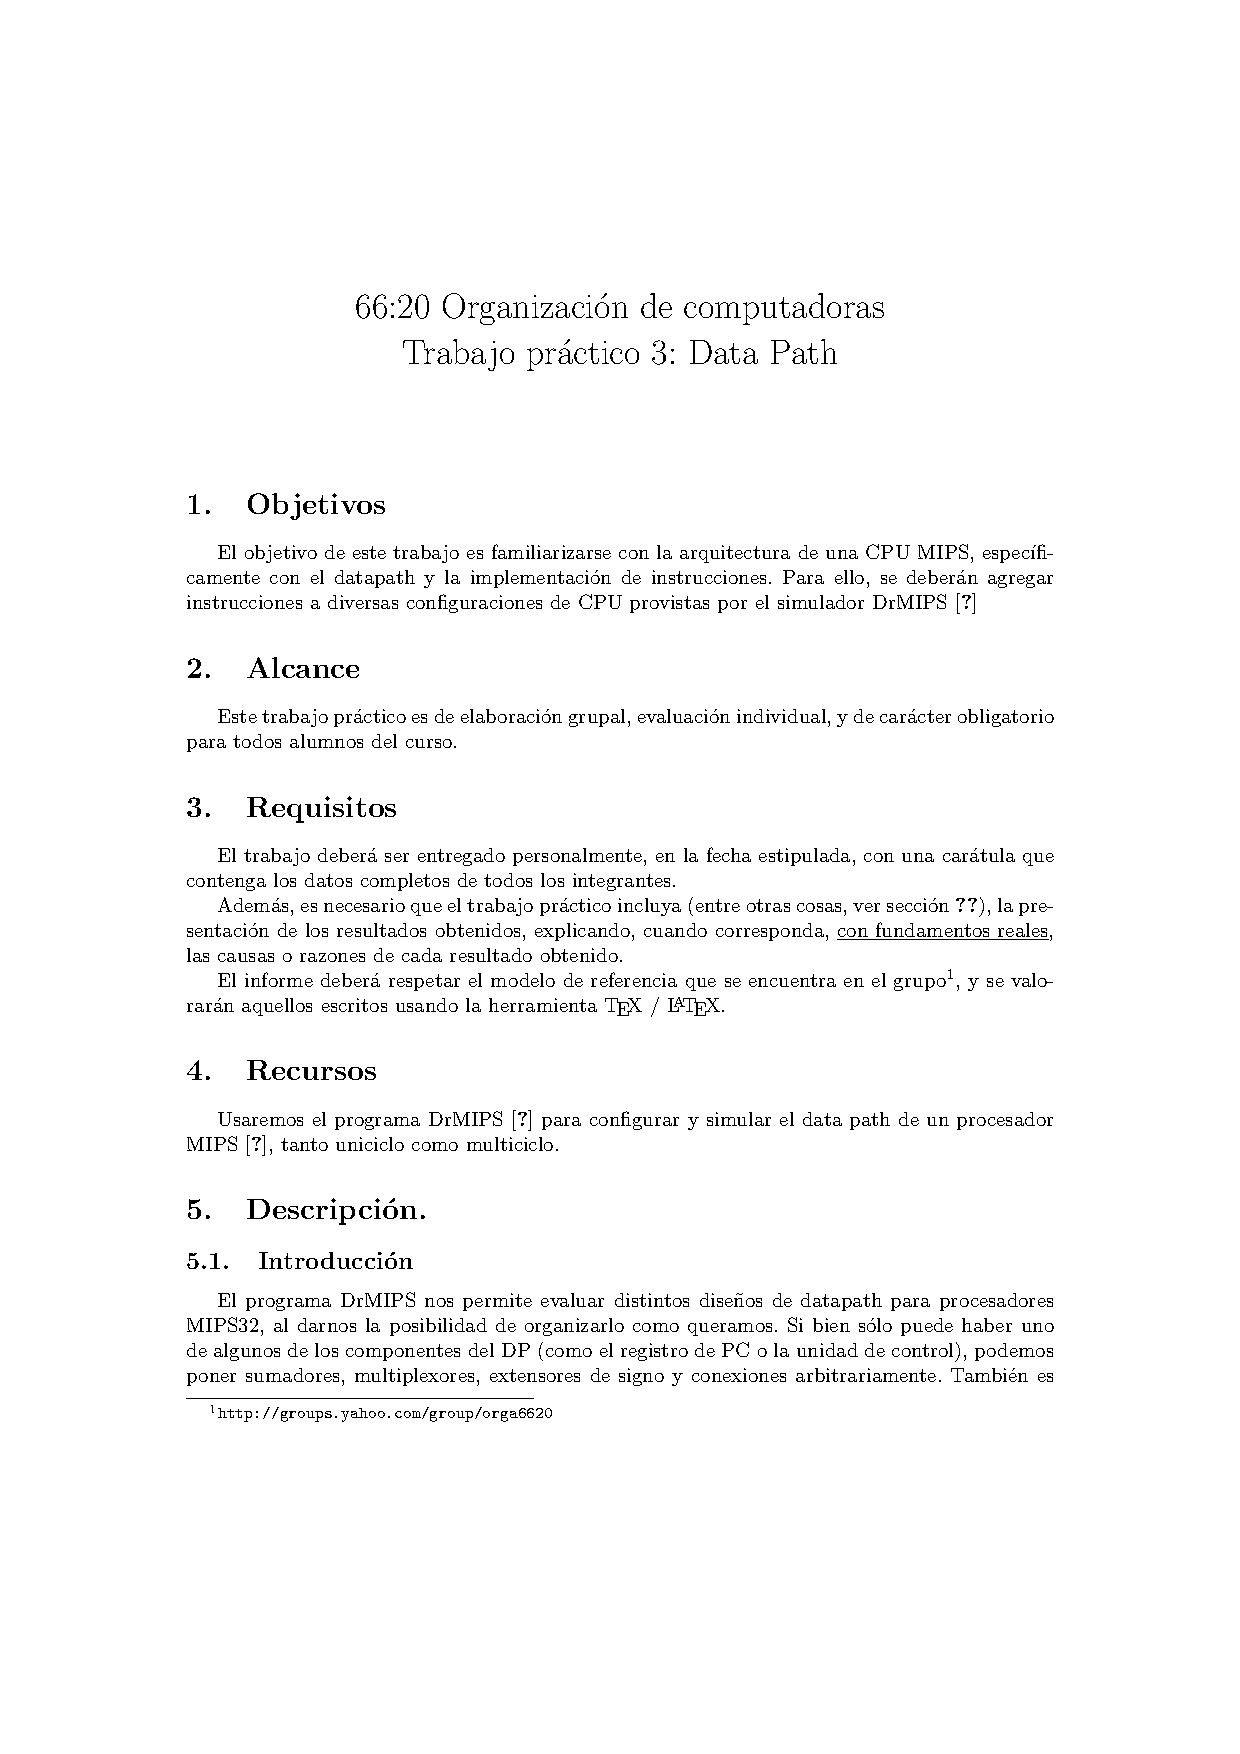
\includepdf[pages=-]{../Enunciado.pdf}

\end{document}
